\documentclass{report}

\usepackage{amsmath}
\usepackage{bookmark}
\usepackage{array} % Included to solve invalid char in Tables declaration
\usepackage{graphicx} % to insert images
\graphicspath{{../pdf/}{/Users/rutviksayankar/Repos/ECE445_SP24/Paperwork/FinalReportLatexEnvironment/Images}} % setting up path for image storage
\usepackage{hyperref} % allows table of contents to be clickable to sections
\hypersetup{
    colorlinks,
    citecolor=blue,
    filecolor=blue,
    linkcolor=blue,
    urlcolor=blue
}

% This section redefines the chapter headings, this allows us to remove the implicit "Chapter #" that comes before a provided chapter title.
\makeatletter
\def\@makechapterhead#1{%
  \vspace*{50\p@}%
  {\parindent \z@ \raggedright \normalfont
    \ifnum \c@secnumdepth >\m@ne
      %\if@mainmatter
        %\huge\bfseries \@chapapp\space \thechapter
        \Huge\bfseries \thechapter.\space%
        %\par\nobreak
        %\vskip 20\p@
      %\fi
    \fi
    \interlinepenalty\@M
    \Huge \bfseries #1\par\nobreak
    \vskip 40\p@
  }}
\makeatother

\title{ECE 445: Senior Design Project Laboratory \\ Final Report \\ Oxygen Delivery Robot} % Sets article title

\author {
    \textbf{Team 27} \\ 
    \textit{Sayankar, Rutvik}\\
    \textit{rutviks2@illinois.edu} \\
    \hfill \\ 
    \textit{Dunican, Aidan}\\
    \textit{dunican2@illinois.edu} \\
    \hfill \\ 
    \textit{Kalyniouk, Nazar}\\
    \textit{nazark2@illinois.edu} \\
    \hfill \\ 
    \textbf{Teaching Assistant} \\ 
    \textit{Subramaniam, Selva} \\
    \textit{ss170@illinois.edu} 
} 
\date{\today} % Sets date for date compiled

% The preamble ends with the command \begin{document}
\begin{document}
    \maketitle % creates title using information in preamble (title, author, date)

    \begin{abstract}
        Mobile oxygen delivery is a mostly untapped market for users both elderly and young. This report details a prototype design for a mobile oxygen delivery robot. We utilize a three wheeled omni-directional drivetrain, ultra wideband triangulation, computer vision, and a simple Roomba style bumper system. We remove ourselves from the context of dealing with oxygen related tubing as swivel solutions already exist and focus on the issue of creating a robot that can autonomously and efficiently move an oxygen tank around in an indoor space.
    \end{abstract}
    
    \pagebreak
    \tableofcontents % creates table of contents
    \pagebreak

    \chapter{Introduction}
    \section{Project Overview}
    Children's interstitial and diffuse lung disease (ChILD) is a collection of diseases or disorders. These diseases cause a thickening of the interstitium (the tissue that extends throughout the lungs) due to scarring, inflammation, or fluid buildup \cite{ChILD-2022}. This eventually affects a patient’s ability to breathe and distribute enough oxygen to the blood. Numerous children experience the impact of this situation, requiring supplemental oxygen for their daily activities. It hampers the mobility and freedom of young children, diminishing their growth and confidence. Moreover, parents face an increased burden, not only caring for their child but also having to be directly involved in managing the oxygen tank as their child moves around.

    Given the absence of relevant solutions in the current market, our project aims to ease the challenges faced by parents and provide young children the freedom to explore their surroundings without worry. As a proof of concept for an affordable solution, we propose a three wheeled omni-directional mobile robot capable of supporting a filled M-6 oxygen tank. We plan to implement two localization subsystems to ensure redundancy and enhance child safety. The first subsystem utilizes Ultra-Wideband (UWB) transceivers for triangulating the child's location relative to the robot in indoor environments, this is similar to how Apple AirTags triangulate their location relative to an iPhone \cite{airtag_uwb} (although AirTags use a combination of UWB and Bluetooth triangulation \cite{airtag_ble}). The second subsystem makes use of a desktop web camera which streams video to a Raspberry Pi where it will leverage open-source object tracking libraries to improve our directional accuracy in tracking a child. The final subsystems will focus on close range object detection.

    \newpage

    \section{Block Diagram}
    \begin{figure}[ht!]
      \centering
      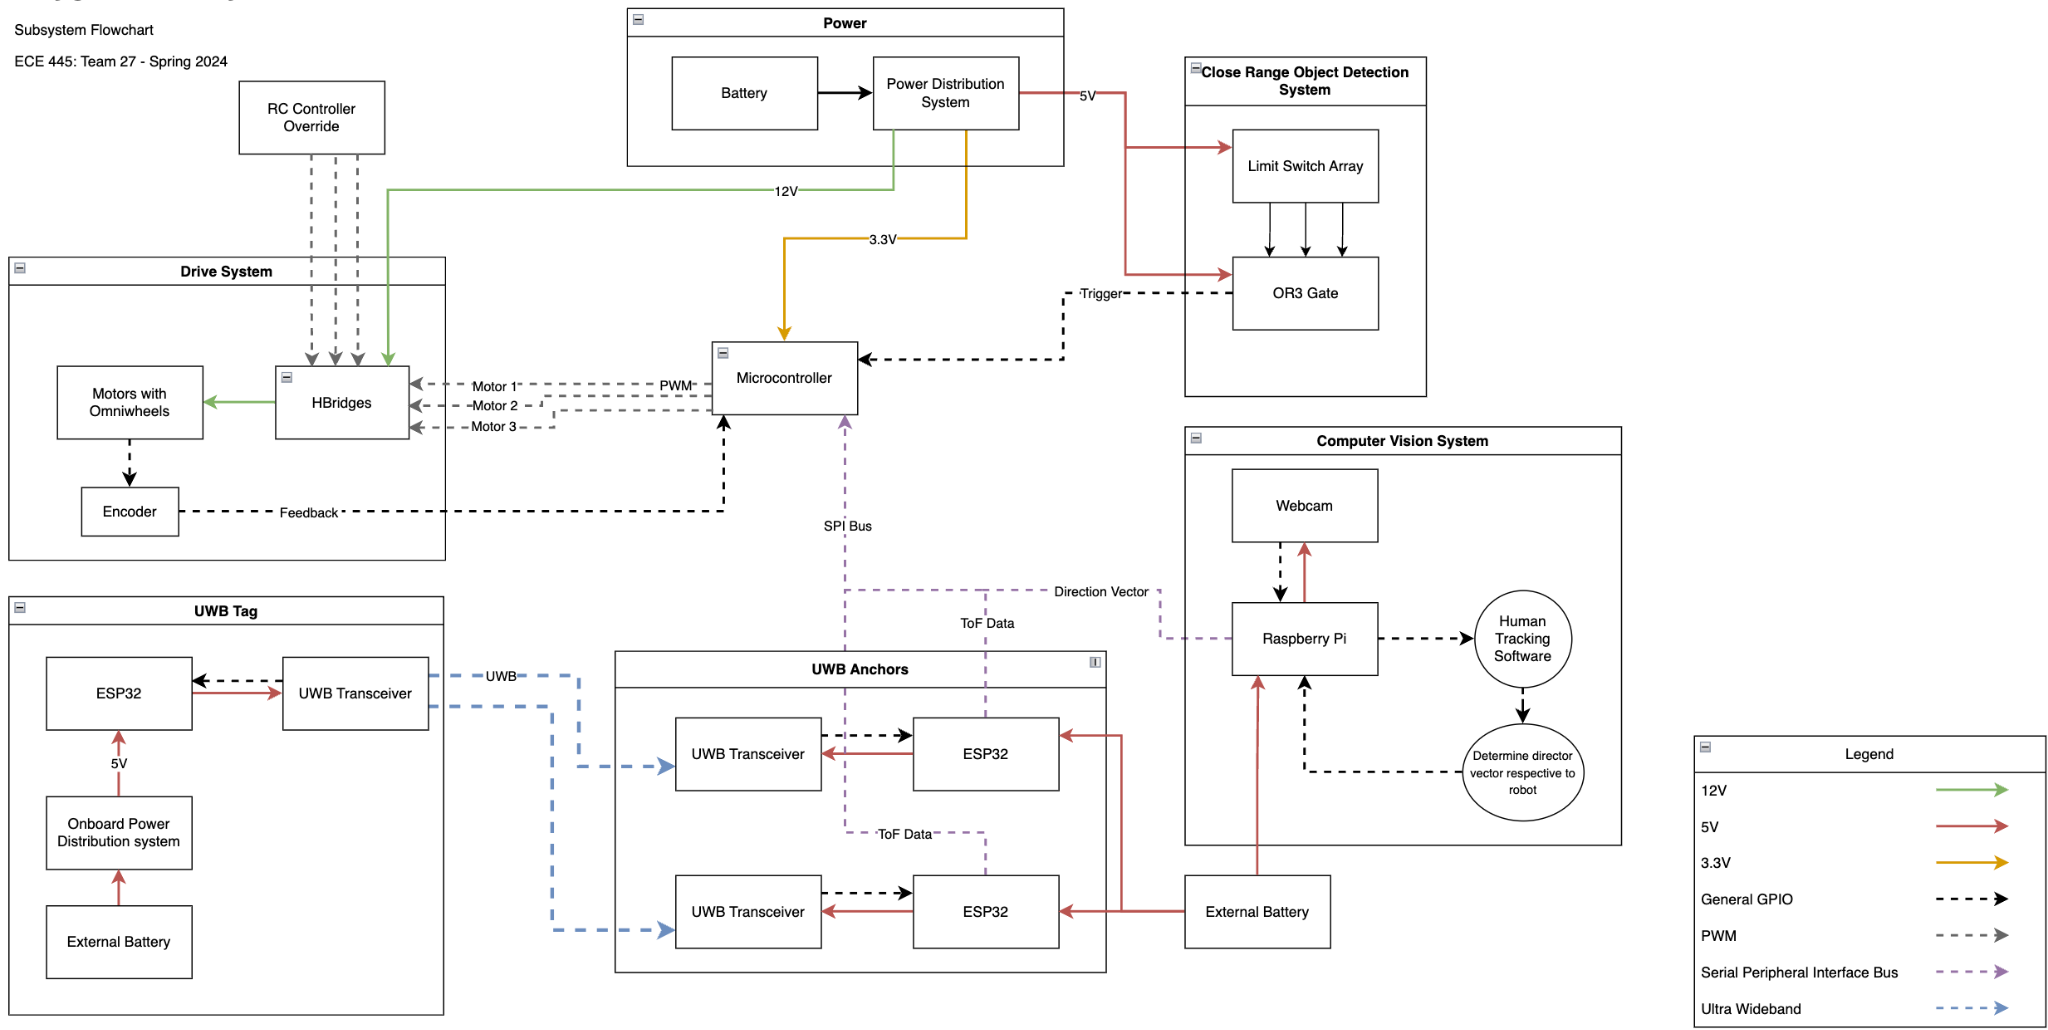
\includegraphics[width=1.2\textwidth]{Images/BlockDiagram.png}
      \caption{High Level Block Diagram}
      \label{fig:BlockDiagram}
  \end{figure}

    \subsection{Omniwheel Drivetrain System}
    We utilize a three wheeled omni-directional wheel drive train. In software we make use of simple matrix multiplication (detailed in section \ref{sec:Omniwheel-InverseKinematics}) to derive individual wheel speeds given that we know where we want to go in Cartesian space.

    \subsection{Ultra-Wideband Triangulation System}
    This system makes use of UWB transceivers in order to triangulate location in an indoor space with high accuracy. The goal was to be able to locate the user in an indoor environment where there maybe be interference with other bluetooth or wifi signals. 
    
    
    
    \subsection{Close Range Object Detection System}
    The Close Range Object Detection subsystem makes use of limit switches with bumpers attached to them arranged in a ring around the robot that will detect when it encounters an object in its path. The goal of this system is to halt the robot and any further movement when a limit switch is pressed. This enhances the safety of the robot, particularly in environments with children. With the expectation that the robot will be utilized inside spaces such as a living room which might have toys scattered around due to younger children being present. To limit the scope of the project we want the robot to simply stop movement upon collision with any object in it's path and have either the user or a someone supervising come in and clear the area before the robot is to be used again.
    
    \subsection{Computer Vision System}
    The Computer Vision subsystem was incorporated into our design to ensure redundancy and robustness. By having a sensor fusion between this and the UWB subsystem, we can ensure that the robot follows the child as desired and add an extra layer of redundancy and safety to our design. The performance requirements of this subsystem are that this subsystem will initiate a corrective measure to the STM32 microcontroller if the child deviates too far from the center of the input frame. Specifically, this system focuses on the degrees away from the center the user currently is. Between the start of this design and the end, nothing was changed in the block level of this subsystem.
    
    \subsection{Control System}
    General Overview on system here
    
    \subsection{Power System}
    General Overview on system here


    \chapter{Design}
    \section{Design Procedure}

    \subsection{Omniwheel Drivetrain System}
    \label{sec:Omniwheel-DesignProcedure}
    Discuss your design decisions for each block at the most general level: What alternative approaches to the design are possible, which was chosen, and why is it desirable? Introduce the major design equations or other design tools used; show the general form of the circuits and describe their functions.

    We utilize a three wheeled omni-directional wheel drive train. Chosen mainly due to the cost benefit over a similar four wheeled drive train. This type of system is susceptible to drift in the form of yaw, therefore we include feedback from encoders back into our STM32 microcontroller to allow for drift compensation.

    \subsubsection{Inverse Kinematics of the OWB}
    \label{sec:Omniwheel-InverseKinematics}
    In a three-wheeled omni-wheel robot, the three wheels are arranged in a triangular pattern, with one wheel at the front and two wheels at the back. Each wheel has several small omni-directional wheels arranged in a circular pattern, which allows the robot to move in any direction.
    
    To move the robot, each wheel is driven independently using a motor. By varying the speed and direction of each wheel, the robot can move in any direction and rotate around its center point.
    
    The kinematics of a three-wheeled omni-wheel robot can be modeled mathematically the below equations \cite{riky2021omnidirectional} which relate the robot's linear and angular velocities to the speed and direction of each wheel.
    
    We first define for each wheel a direction of rotation $V_i$, and the resulting movement effected in the x and y axes, $V_ix$ and $V_iy$ as shown below.

    \begin{figure}[ht!]
      \centering
      \begin{minipage}[b]{0.45\linewidth}
        \centering
        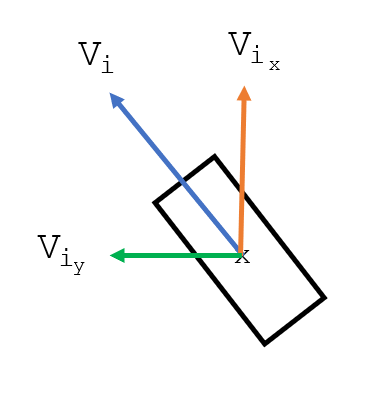
\includegraphics[width=\linewidth]{wheel_vector.png}
        \caption{Vector Definitions}
        \label{fig:vecdef}
      \end{minipage}
      \hfill
      \begin{minipage}[b]{0.45\linewidth}
        \centering
        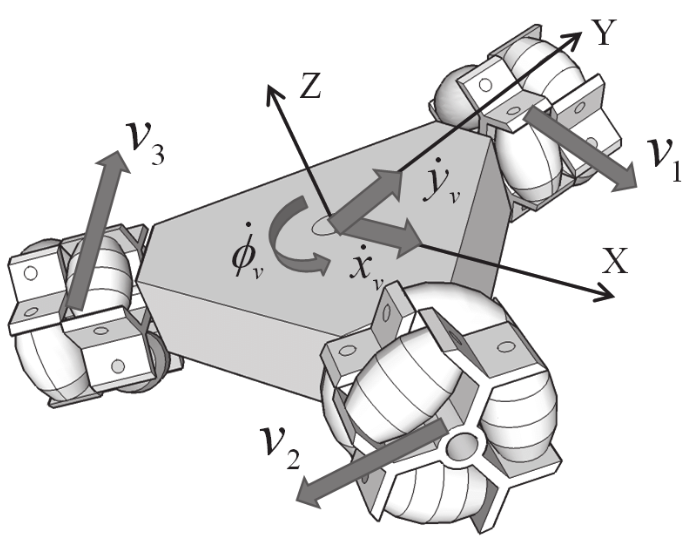
\includegraphics[width=\linewidth]{OWB_vectors.PNG}
        \caption{OWB drive vectors \cite{wada2015OWB}}
        \label{fig:owb_vec}
      \end{minipage}

      \label{fig:vecs}
    \end{figure}

    Knowing the angle of each wheel from the vertical axis, we can compute the x and y components created by the rotation of each wheel. By summing these components together, we can get the effective motion of the robot in the x, y and yaw axes.
    
    \[
    \begin{pmatrix}
    V_x \\
    V_y \\
    \omega
    \end{pmatrix}
    =
    \begin{pmatrix}
    1 & - \frac{1}{2} & -\frac{1}{2} \\
    0 & -\frac{\sqrt{3}}{2} & \frac{\sqrt{3}}{2} \\
    1 & 1 & 1
    \end{pmatrix}
    \begin{pmatrix}
    V_1 \\
    V_2 \\
    V_3
    \end{pmatrix}
    \]
        
    $V_{x}$ and $V_{y}$ are the desired linear velocities in the x and y directions, respectively, and omega is the desired angular velocity. $V_{1}$, $V_{2}$, and $V_{3}$ are the velocities of the three wheels, and L is the distance between the robot's center of mass and the wheel axes.

    \[
    \begin{pmatrix}
    V_1 \\
    V_2 \\
    V_3
    \end{pmatrix}
    =
    \begin{pmatrix}
    1 & - \frac{1}{2} & -\frac{1}{2} \\
    0 & -\frac{\sqrt{3}}{2} & \frac{\sqrt{3}}{2} \\
    1 & 1 & 1
    \end{pmatrix}^{-1}
    \begin{pmatrix}
    V_x \\
    V_y \\
    \omega
    \end{pmatrix}
    \]

    By taking the inverse of our 3x3 component coefficient matrix above, we can solve for our individual motor speeds $V_1$, $V_2$ and $V_3$, given the desired motion in terms of $V_x$, $V_y$, and $w$.

    \subsection{RC Control}
    For drivetrain testing and part of our demo we used an RC controller. We made use of a Flysky FS-i6 6CH 2.4GHz Radio System RC Transmitter Controller with FS-iA6 Receiver. While the receiver supports up to six channels, the OWB only needs three channels. 

    The OWB can move forward and backward like a normal RC car. This motion is represented by $V_y$, and is mapped to CH1 on the transmitter. While a normal RC car needs a $V_y$ component to turn left or right, the OWB can "yaw" on the spot. This is represented by $w$, and is mapped to CH3 on the transmitter. The final unique motion the OWB can execute is a "drift" toward the left or right. This motion is represented by $V_x$ and is mapped to CH2 on the transmitter.

    Thus, using these three channels, the operator can define the robot's desired $V_x$, $V_y$, and $w$. These desired motion vectors are then fed to our inverse kinematics algorithm, which breaks down our desired motion into an individual wheel speed and direction for each motor.

    \begin{figure}[ht!]
    \begin{center}
        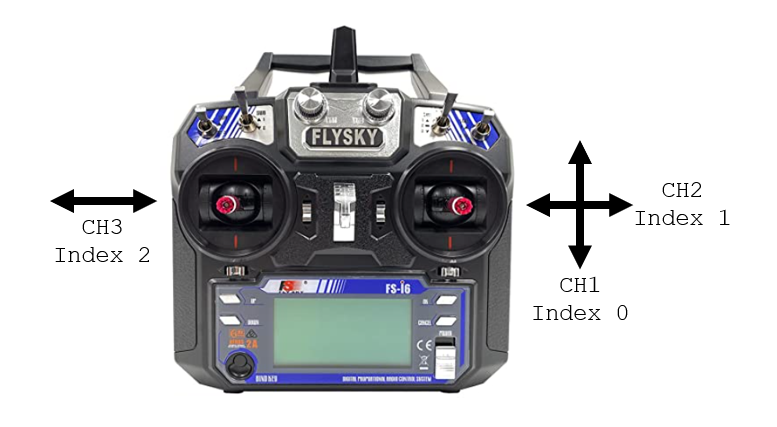
\includegraphics[width=0.8\textwidth]{channel.PNG}\\
        \caption{ Channel Distribution  } 
        \label{}
    \end{center}
    \end{figure}
    

    \subsection{Ultra Wideband Triangulation System}
    Our initial design discussion was regarding the type of wireless indoor localization we want to design. Immediately, two types of communication came to mind: UWB and BLE. Ultimately, we chose UWB over BLE due to the following benefits:

    \begin{itemize}
      \item Data transmission: UWB can transmit more data than Bluetooth Low Energy
      \item Accuracy: UWB can more accurately measure distance and determine position because it uses wideband radio waves and higher frequency bands
      \item Interference resistance: UWB is less likely to be affected by interference and obstructions
    \end{itemize}

    \subsubsection{Localization Algorithms} 
    To break it down simply, our goal was to find out the location of a user relative to our robot. We assume the user and robot will be in a valid location in real world space, and therefore can just focus on the user's location relative to our robot.

    To localize the user, we need to create a triangle of known lengths with vertices defined by the UWB transceivers. To obtain the lengths of each side we need to perform some ranging between the tag transceiver (the transceiver which the user will have) and the anchor transceivers (which are mounted onto the robot). With the anchors being a set 18" apart (the minimum as required by the DW3000 ICs we were using), we only needed the remaining two sides of our triangle.

    There are two ways to range between UWB transceivers. The first is to use Time of Flight (ToF). ToF is a positioning method based on two-way ranging. That means the tag needs to send and receive signals from the anchor several times and then the flight time of the signal between the anchor and the tag can be measured, because radio waves travel at the speed of light, we can calculate the distance between the tag and each anchor given that we know how long it took for a signal to travel between them. Secondly, Time Difference of Arrival (TDoA) is localization based on comparing the time difference between signals and each anchor and this technique requires an accurate time synchronization function. When using the TDoA method, the UWB tag will send out a poll message, and all the nearby UWB anchors will receive it and record the arrival time. Because the location of anchors is different, they will not receive the message at the same time. We can use these time differences to determine the tag’s location.

    Implementing an accurate time synchronization function between all of our transceivers increases the complexity of the project ten-fold therefore we decided to use a ToF based ranging method to calculate the distance between each anchor and the tag device.
    
    \subsection{Close Range Object Detection System}
    Discuss your design decisions for each block at the most general level: What alternative approaches to the design are possible, which was chosen, and why is it desirable? Introduce the major design equations or other design tools used; show the general form of the circuits and describe their functions.

    This system is the simplest but definitely required some debate in terms of how we wanted it implemented. We debated between two main types of detection: simple limit switches or ultrasonic sensors. Limit switches don't require explanation, you activate a switch and a signal goes high. The only struggle here would be finding a limit switch that would be suitable for our needs. The alternative was ultrasonic detection which would have required us to use a much larger number of sensors and which would have been much more sensitive. The reason we decided to use limit switches was that they would only stop the robot when an object collides with it. In addition, limit switches allow us to make a 360-degree bumper for the robot with only 3 switches, which would fill in the gap between each wheel. To design the subsystem we decided to go with the 3 Honeywell 101SN11 limit switches as they were the best available limit switch in the ECE Self-service center (put simply, it was the only limit switch that could take any sort of impact without damage). One of the major issues we had when designing this subsystem was how to get the Honeywell limit switches to work. Seeing as these limit switches have since been discontinued, finding proper documentation on them proved to be difficult. We discovered that the output to the limit switches needed a 10k pull-up resistor in order to drive the output high when the limit switch is inactive. This was all thanks to a helpful ebay seller who provided a simple explanation on the function of some old limit switches he was selling (\url{www.ebay.com/itm/333999755279 }).
    
    \subsection{Computer Vision System}
    Discuss your design decisions for each block at the most general level: What alternative approaches to the design are possible, which was chosen, and why is it desirable? Introduce the major design equations or other design tools used; show the general form of the circuits and describe their functions.
    
    \subsection{Control System}
    Discuss your design decisions for each block at the most general level: What alternative approaches to the design are possible, which was chosen, and why is it desirable? Introduce the major design equations or other design tools used; show the general form of the circuits and describe their functions.
    
    \subsection{Power System}
    Discuss your design decisions for each block at the most general level: What alternative approaches to the design are possible, which was chosen, and why is it desirable? Introduce the major design equations or other design tools used; show the general form of the circuits and describe their functions.

    \section{Design Details}

    \subsection{Omniwheel Drivetrain System}
    Present the detailed design, with diagrams and component values. Show how the design equations were applied. Give equations and diagrams with specific design values and data. Place large data tables in an appendix. Circuit diagrams that are too large to be readable on a single page should be broken into pieces for presentation. The full diagram may be included in an appendix. Use photographs only as necessary and treat them, along with all other graphics except tables, as figures.

    \subsection{Ultra Wideband Triangulation System}
    Present the detailed design, with diagrams and component values. Show how the design equations were applied. Give equations and diagrams with specific design values and data. Place large data tables in an appendix. Circuit diagrams that are too large to be readable on a single page should be broken into pieces for presentation. The full diagram may be included in an appendix. Use photographs only as necessary and treat them, along with all other graphics except tables, as figures.

    \subsection{Close Range Object Detection System}
    Present the detailed design, with diagrams and component values. Show how the design equations were applied. Give equations and diagrams with specific design values and data. Place large data tables in an appendix. Circuit diagrams that are too large to be readable on a single page should be broken into pieces for presentation. The full diagram may be included in an appendix. Use photographs only as necessary and treat them, along with all other graphics except tables, as figures.

    \subsection{Computer Vision System}
    Present the detailed design, with diagrams and component values. Show how the design equations were applied. Give equations and diagrams with specific design values and data. Place large data tables in an appendix. Circuit diagrams that are too large to be readable on a single page should be broken into pieces for presentation. The full diagram may be included in an appendix. Use photographs only as necessary and treat them, along with all other graphics except tables, as figures.

    \subsection{Control System}
    Present the detailed design, with diagrams and component values. Show how the design equations were applied. Give equations and diagrams with specific design values and data. Place large data tables in an appendix. Circuit diagrams that are too large to be readable on a single page should be broken into pieces for presentation. The full diagram may be included in an appendix. Use photographs only as necessary and treat them, along with all other graphics except tables, as figures.  

    \subsection{Power System}
    Present the detailed design, with diagrams and component values. Show how the design equations were applied. Give equations and diagrams with specific design values and data. Place large data tables in an appendix. Circuit diagrams that are too large to be readable on a single page should be broken into pieces for presentation. The full diagram may be included in an appendix. Use photographs only as necessary and treat them, along with all other graphics except tables, as figures.

    \chapter{Verification}

    Discuss the testing of the completed project and its major blocks. Provide solid technical data, and present it in an easily grasped manner, using graphs where necessary. Include any standard tests for your type of circuit and all specific ones you feel are needed to prove that the design goals were met. Discuss the Requirement and Verification Table from your design review. Including the table in an appendix will help avoid lengthy and tedious narrative description in the main text, which may not be of immediate interest to your imagined audience of managers. Do not discuss low-level requirements unless they failed to verify, or you found that they were critical in some unexpected way, or you need to makes changes—for instance, to the tolerances or acceptable ranges of quantitative results. It is important to hit the main points and explain any requirement that is not verified, but keep the discussion concise and refer interested readers to the appendix for details.

    \section{Omniwheel Drivetrain System}
    Verification details on the system here

    \section{Ultra Wideband Triangulation System}
    Verification details on the system here
    
    \section{Close Range Object Detection System}
    Verification details on the system here
    
    \section{Computer Vision System}
    Verification details on the system here
    
    \section{Control System}
    Verification details on the system here
    
    \section{Power System}
    Verification details on the system here

    \chapter{Costs}

    Labor cost estimates should use the following formula for each partner: ideal salary (hourly rate) = actual hours spent * 2.5 
    
    Include estimates for electronics and machine shop hours, as applicable. For parts, use real values when you know them; make realistic estimates otherwise. List both the retail cost and what you or the department paid (in this case you may list lab-owned pieces as free). If the project might be commercially viable, estimate the cost of mass-production by listing bulk-purchase costs. Make sure any tables are numbered appropriately, given titles, and cited directly in the text. 

    \begin{center}
      \begin{tabular}{ | m{10em} | m{4em} | m{10em} | } 
        \hline
        Item & Quantity & Cost  \\ 
        \hline
        \hline
        PCB BOM
        & 
        1
        &
        \$62.03
        \\ 
        \hline
        PCB Manufacturing
        & 
        1
        &
        \$40.38
        \\ 
        \hline
        3D Printing 
        &
        1
        &
        \$5
        \\
        \hline
        \href{https://www.andymark.com/products/4-in-duraomni-wheel}{Omni-Wheels}
        &
        3
        &
        \$78
        \\
        \hline
        \href{https://www.gobilda.com/modern-robotics-12vdc-motor/}{Modern\:Robotics 12VDC Motor}
        &
        3
        &
        \$44.97
        \\
        \hline
        \href{https://www.digikey.com/en/products/detail/jst-sales-america-inc/B4B-XH-A/1651047}{4-pin connector}
        &
        7
        &
        \$1.61
        \\
        \hline
        \href{https://www.gobilda.com/4-pos-jst-ph-mh-fc-to-4-pos-jst-xh-mh-fc-adaptor-150mm-length/}{4-pin jumper cable}
        &
        4
        &
        \$11.56
        \\
        \hline
        \href{https://www.team358.org/files/programming/ControlSystem2015-2019/specs/217-2769-Victor888UserManual.pdf}{Victor 888 Speed Controller}
        &
        3
        &
        \$149.97
        \\
        \hline
        \href{https://www.amazon.com/Logitech-Internet-Camera-2-0-Megapixel-Resolution/dp/B000RZQZM0}{QuickCam Pro 9000}
        &
        1
        &
        \$74.99
        \\
        \hline
        \href{https://www.makerfabs.com/esp32-uwb-dw3000.html}{ESP32UWB DW3000(Ultra-Wideband transceiver)}
        &
        3
        &
        \$131.40
        \\
        \hline
        \href{https://vilros.com/products/raspberry-pi-4-model-b}{Raspberry\:Pi\:4\:1GB Model B}
        &
        1
        &
        \$35
        \\
        \hline
        Total
        &
        &
        \$634.91
        \\
        \hline
      \end{tabular}
    \end{center}

    \chapter{Conclusions}

    Bring together, concisely, the conclusions to be drawn. It may be appropriate, depending on the nature of the project, to begin or end with a two- or three-sentence executive summary. The reader needs to be convinced that the design will work. Summarize your accomplishments. If uncertainties remain, they should be pointed out, and alternatives, such as modifying performance specifications, should be spelled out to deal with foreseeable outcomes. Use words, not equations or diagrams. Devote a section to ethical considerations with reference to the IEEE Code of Ethics and any other applicable code (e.g., the AMA Code of Medical Ethics for certain bioengineering projects). Either here or in the background discussion of your introduction, provide a paragraph addressing the broader impacts of your project in terms of global, economic, environmental and/or societal contexts.

    \section{Ethics and Safety}
    \subsection{Ethical Considerations}
    As we continue through the development of our project, we are unwavering in our dedication to abide by the ethical and safety principles outlined by the Association for Computing Machinery (ACM) and the Institute of Electrical and Electronics Engineers (IEEE). As we embark on this project, we pledge our commitment to adhere to these standards, ensuring that our actions and choices uphold the highest level of professionalism and integrity.

    As outlined in Section I of the IEEE Code of Ethics, we pledge to “uphold the highest standards of integrity, responsible behavior, and ethical conduct in professional activities” \cite{IEEE_2020}. We will prioritize safety in our design and adhere to ethical design practices. Educating the parents and caregivers about the robot’s use and limitations will allow for informed decision-making. Following relevant laws and regulations regarding this technology will also be a high priority.

    In the same Code of Ethics, outlined in Section III, we pledge to “strive to ensure this code is upheld by colleagues and co-workers” \cite{IEEE_2020}. We will support each other in ethical conduct and foster a culture of ethical behavior. Open communication will be established and encouraged to raise concerns and provide guidance to team members.

    \subsection{Safety Considerations}
    This project aligns with the safety principles outlined in the ACM Code of Ethics and Professional Conduct. Safety remains our number one priority and as outlined in Section 1.2 \cite{ACM_2018}, we will avoid negative consequences, especially when those consequences are significant and unjust. We will take careful consideration of potential impacts and minimize harm. In the context of this project, we will ensure that the robot’s design and operation prioritizes safety, especially to the children this product aims to assist. We will work to analyze potential risk and consider the robot’s mobility and interaction with its environment.

    As well as promoting safety, privacy is also a very important guideline that will be followed, which is outlined in Section 1.6. As professionals, we must safeguard the personal information of our users, especially if it involves children. As it relates to this project, we will ensure that no data will be collected and stored in an external location. Data collection will be minimized to only what is necessary for the robot to operate.

    One aspect of our project where safety must be considered is regarding the use of lithium batteries. We acknowledge the potential risks associated with the misuse of lithium batteries. We are committed to following the safety guidelines associated with the batteries we plan on using. More specifically, maintaining the battery’s temperature within the recommended range. Also, we are dedicated to the responsible disposal of batteries to ensure sustainability.

    Since we are incorporating motors into our design, we will deploy essential control systems to mitigate potential hazards such as collisions with the environment. Safe operation will be ensured with the use of sensors, vision systems, and warning systems.

    \appendix

    \chapter{Appendix}

    \section{Terms and Keywords}
    \begin{itemize}
        \item ChILD - Children's Interstitial and Diffuse Lung Disease
        \item PCB – Printed Circuit Board
        \item OWB - Three-Wheeled Omni-Wheel Bot
        \item UWB - Ultra-wideband is a radio technology that can use a very low energy level for short-range, high-bandwidth communications over a large portion of the radio spectrum.
        \item ESP32 - A series of low-cost, low-power system-on-a-chip microcontrollers with integrated Wi-Fi and dual-mode Bluetooth.
        \item RPM - Revolutions per minute
        \item GPIO - General-purpose input/output
        \item SPI - Serial Peripheral Interface
        \item PWM - Pulse-width modulation
        \item MPH - Miles per hour
        \item OpenCV - (Open Source Computer Vision Library) is an open source computer vision and machine learning software library.
        \item TDoA - Time Difference of Arrival 
        \item ToF - Time of Flight
        \item BOM - Bill of materials
    \end{itemize}

    \bibliographystyle{IEEEtran}
    \bibliography{ref}

\end{document} % This is the end of the document